\setcounter{exo}{0}

On s'intéresse à la liaison entre l'axe de la toue et le châssis du véhicule. Les notations adoptées seront les suivantes : $F^a_{C}$ (respectivement $F^r_{C}$, $F^x_{C}$) désignera la composante suivant $\vect{a}$ (respectivement $\vect{r}$, $\vect{x}$) de l'effort extérieur exercé en $C$. On procédera de même pour le point $D$. 
\begin{center}
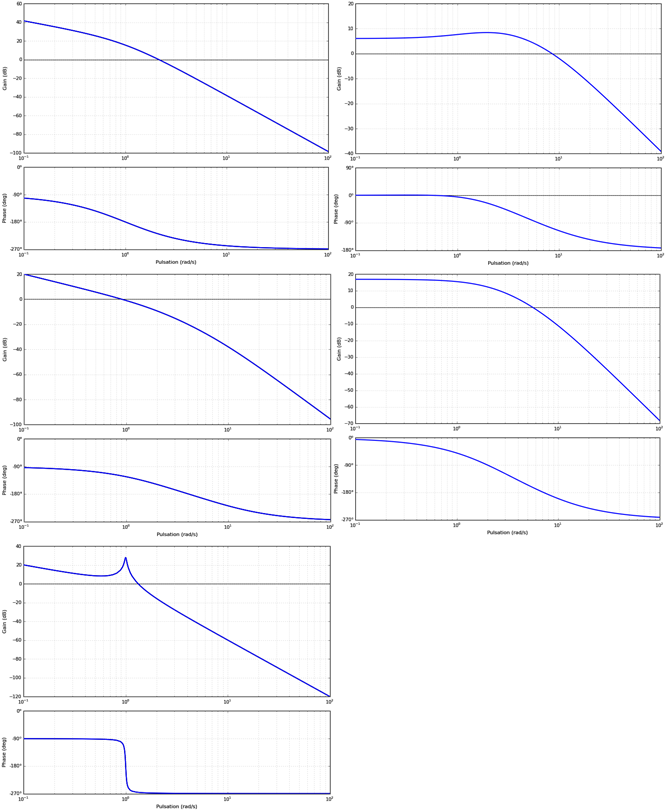
\includegraphics[width=\linewidth]{fig_01}
\end{center}


\subparagraph{}\textit{En isolant l'ensemble \{pneumatique + jante + axe de roue\}, écrire les équations issues du principe fondamental de la statique appliqué au point $C$, en projection sur les axes de la base $\base{a}{r}{x}$ en fonction des composantes $F_{\text{sol}}^a$ et $F_{\text{sol}}^r$ et des dimensions $d_0$, $d_3$ et $d_4$.}

\subparagraph{}\textit{Peut-on résoudre complètement le système ? Pourquoi ?}

\subparagraph{}\textit{Résoudre littéralement le système.}